\documentclass[11pt,a4paper]{article}
\usepackage{amsthm,amsmath,amsfonts,exscale,latexsym,graphicx,dsfont}
\usepackage{times}
%\usepackage[mtpcal,mtphrb,subscriptcorrection]{mtpro2}
\usepackage{natbib}
\usepackage[usenames]{color}
\usepackage[pagebackref,colorlinks=true,breaklinks,linkcolor=Gray,citecolor=Gray,urlcolor=Gray,bookmarks,pdfpagemode=UseOutlines,pdftitle={Deep Learning Project 2019: Round Trip Loss for Machine Translation}]{hyperref}
\graphicspath{ {./images/} }
\usepackage[a4paper, total={6in, 8in}]{geometry}


\bibliographystyle{apalike}
%shortcuts
\def\beq{\begin{equation}}
\def\eeq{\end{equation}}
\begin{document}
\title{Deep Learning Lecture 2019 - Project:\\Round Trip Loss for Machine Translation}
\date{\today}
\author{
Anja Adamov$\mbox{}^a$\thanks{\emph{E-mail address:} adamova@student.ethz.ch},
Lauro B\"{o}ni$\mbox{}^b$\thanks{\emph{E-mail address:} laboeni@gmail.com},
Simon A.\ Broda$\mbox{}^c\mbox{}^d\mbox{}^e$\thanks{\emph{E-mail address:} simon.broda@uzh.ch},
Urs V\"{o}geli$\mbox{}^b$\thanks{\emph{E-mail address:} voegeli.urs@gmail.com}
\medskip \\
\textit{\small $\mbox{}^a$IBM Switzerland Ltd., Zurich, Switzerland}
\medskip \\
\textit{\small $\mbox{}^b$ETH Zurich}
\medskip \\
\textit{\small $\mbox{}^c$Department of Banking and Finance, University of Zurich}
\medskip \\
\textit{\small $\mbox{}^d$Quantitative Economics Section, University of Amsterdam}
\medskip \\
\textit{\small $\mbox{}^e$Tinbergen Institute Amsterdam}
}
\maketitle \setcounter{page}{0}\thispagestyle{empty}
\definecolor{Gray}{rgb}{0.5,0.5,0.5}
\begin{abstract}
We propose to augment a machine translation system by adding a round-trip loss which encourages the system to generate translations that when translated back into the source language, retain much of the original structure. We conjecture that in doing so, the model will learn internal representations with improved semantic meaning.
\end{abstract}
\bigskip \textbf{Key Words}: Cycle consistency loss; deep learning; natural language understanding; machine translation; round-trip loss.
%\renewcommand{\baselinestretch}{1.3}\small\normalsize
\newpage
\setcounter{page}{1}
\section{Introduction}
Machine translation is an important task within the field of natural language understanding. Consequently, a variety of models have been proposed for solving it. One of the first truly successful models was the sequence-to-sequence ({\tt seq2seq}) model of \citet{seq2seq}, while the current state of the art builds upon the \emph{transformer} architecture introduced by \citet{transformer}. At a high level, both the seq2seq and the transformer architectures are comprised of an encoder and decoder; the encoder learns an internal representation of the source sentence, and the decoder decodes it into the target language. For these models to work, the internal representation must capture the semantic meaning of the source sentence.

Irrespective of the architecture, these models are typically trained with the cross-entropy loss between the ground truth and predicted sentences, usually with teacher forcing.

Here, we propose to add a round-trip penalty to the loss function of the model. The idea is that instead of training a single model to translate from a source language $\mathcal{S}$ to a target language $\mathcal{T}$, one trains two models (of identical structure), one mapping $\mathcal{S} \xrightarrow{} \mathcal{T}$ and one mapping $\mathcal{T}\xrightarrow{} \mathcal{S}$. The two models are, at first, trained independently and in parallel by feeding in the same batches of sentence pairs. After $\tau$ epochs, the models will then be trained jointly, using as loss a sum of four cross-entropy terms, viz.,
\begin{equation*}
    \mathcal{L}_{\mathcal{S}, \mathcal{T}} (s,t) = \text{CE}(s, \hat{s}) + \text{CE}(t, \hat{t}) + \lambda \left( \text{CE}(s, \tilde{s}) + \text{CE}(t, \tilde{t}) \right),
\end{equation*}
where $s\in\mathcal{S}$ is the ground truth sentence in the the first language, $t\in\mathcal{T}$ is the corresponding ground truth in the second language, $\hat{s}\in\mathcal{S}$ and $\hat{t}\in\mathcal{T}$ are the respective translations of $t$ and $s$, $\tilde{s}$ is obtained by translating $\hat{t}$ back to $\mathcal{S}$, and $\tilde{t}$ is obtained by translating $\hat{s}$ back to $\mathcal{T}$. $\tau$ and $\lambda$ are hyperparameters. 

The round-trip loss is inspired by the cycle consistency loss pioneered by \citet{CycleGAN2017} in the context of GANs. The only application of this concept to the field of machine translation of which we are aware is \citet{su:2018}, who adapt it for unsupervised multi-modal machine translation. Here, we propose to apply the idea to supervised machine translation. We surmise that encouraging the model to generate round-trippable translations will help it learn a semantically meaningful representation.

%In order to make this idea operational, we will use the seq2seq model implementation at \href{https://github.com/tensorflow/nmt}{https://github.com/tensorflow/nmt} as a starting point, augmenting it with our proposed round-trip loss and training it on the WMT'14 English-German data set available from \href{https://nlp.stanford.edu/projects/nmt/}{https://nlp.stanford.edu/projects/nmt/}, possibly restricting attention to a subset for computational reasons. Hyperparameters will be tuned by cross-validation on the BLEU score \citep{bleu}. Results will be compared to the seq2seq model without round-trip loss as a baseline. Possible extensions include i) replacing the simplistic seq2seq architecture with the state-of-the-art transformer architecture of \citet{transformer}, ii) using pre-trained word embeddings from BERT \citep{bert} rather than learning the embeddings from scratch, (iii) investigating the performance for other language pairs.

\section{Model and Methods}
\subsection{Architecture}
As described in previous sections, we have based our model extension on the transformer model implementation at \textbb{cite}. The core idea behind the classical transformer model is the so-called self-attention — the model's ability to attend to different positions of the input sequence to compute a representation of that sequence. (ref: https://www.tensorflow.org/tutorials/text/transformer)

For deep neural networks performing aiming to perform sequence translation, some general sort of memory is required as, in practice, a lot of sequences depend on words from previous sequences. As an example for the reader, try to complete the phrases "My father is a winegrower. He likes to drink {\tt ...}". In this case, you might guess the missing word "wine" correctly - with the help of attention. And this is exactly, what modern natural language models try to capture.

Recurrent Neural Networks (short: RNN) tackle this problem by a specific architecture that focuses on time-dependencies. However, they are hardly or even not parallelizable and hence computationally suboptimal. 
On the other hand, Convolution Neural Networks (short: CNN) are easily parallelizable and can exploit local dependencies. However, these models do not explicitly focus on the attention part. 

The transformer model is a combination of a CNN together with attention - more precisely with self-attention. In a nutshell, the transformer model consists of a set of encoders (EC) and set of decoders (DC). The ECs map input sequences $(x_1,...,x_n)$ to its continuous representation, say, $(z_1,...,z_n)$ which in turn is used by DCs to generate the output respective the translated prediction $(y_1,...,y_m)$.

More precisely, each EC consists of two components: self-attention and feed-forward neural networks (FNN). The self-attention mechanism takes in a set of input encodings from the previous EC and weighs their relevance to each other to generate a set of output encodings. The FNN then further processes each output encoding individually. These output encodings are finally passed to the next EC as its input, as well as to the DC. \textbf{cite wikipedia}

On the other hand, each DC consists of three components: self-attention, an attention mechanism over the encodings and a FNN. The first EC takes positional information and embeddings of the input sequence as its input, rather than encodings. The positional information is necessary for the transformer to make use of the order of the sequence. Each DC functions in a similar fashion to the ECs, but an additional attention mechanism is inserted which instead draws relevant information from the encodings generated by the EC. Like the first EC, the first DC takes positional information and embeddings of the output sequence as its input, rather than embeddings. The last DC is followed by a final linear transformation and softmax layer, to produce the desired output probabilities.

\begin{figure}[h]
    \centering
    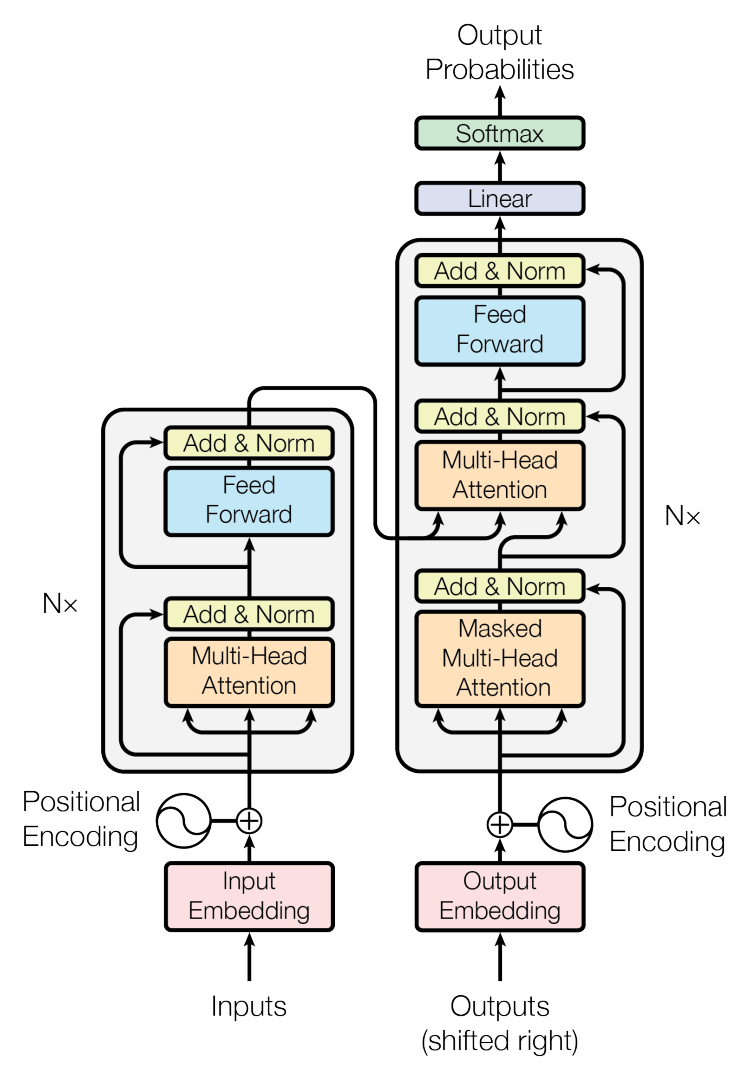
\includegraphics[scale=0.5]{paper/images/Transformer.PNG}
    \caption{Architecture of the Transformer model}
    % cite: https://arxiv.org/pdf/1706.03762.pdf
    \label{fig:transformer}
\end{figure}

This somehow abstract description is visualized in Figure \ref{fig:transformer}, where the original model in (\textbf{cite}) uses $N=6$, i.e. 6-fold stacking of the respective ECs and DCs.

The self-attention part in both the EC as well as DC consists of a quite involved procedure that, in a nutshell, learns contextual dependencies. The authors of \textbf{cite} visualized the attention part by Figure \ref{fig:attention}:

\begin{figure}[h]
    \centering
    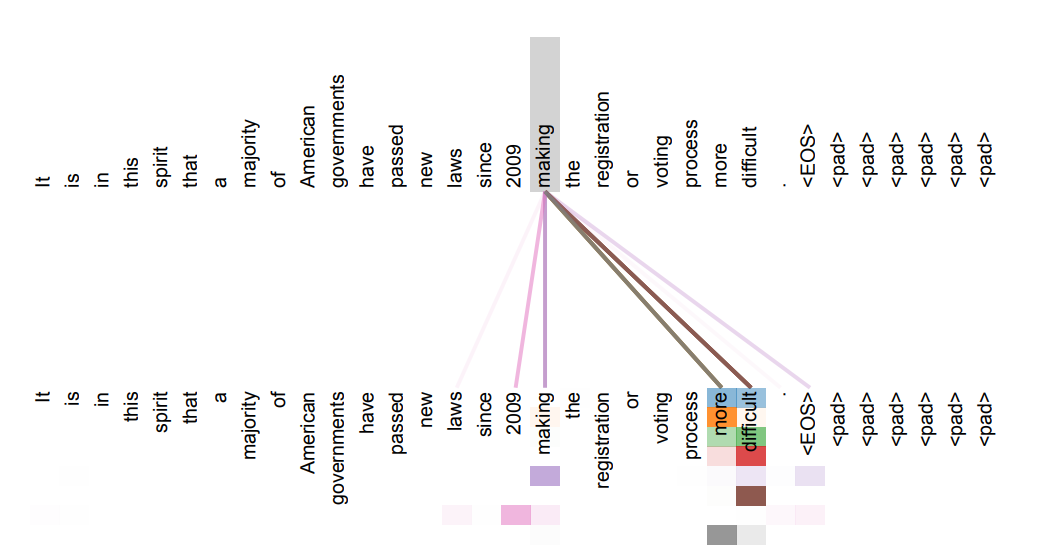
\includegraphics[scale=0.7]{paper/images/attention.PNG}
    \caption{Visualization of the self-attention mechanism.}
    % cite: https://arxiv.org/pdf/1706.03762.pdf
    \label{fig:attention}
\end{figure}

For a detailed description of the attention mechanism, we refer to \textbf{cite} (original paper) or \href{some interesting url}{some interesting url}.

\textbf{to-be-continued}
\cite{http://jalammar.github.io/illustrated-transformer/}


\href{https://en.wikipedia.org/wiki/Transformer_(machine_learning_model)#Architecture}{https://en.wikipedia.org/wiki/Transformer_(machine_learning_model)#Architecture}

\href{https://towardsdatascience.com/transformers-141e32e69591}{https://towardsdatascience.com/transformers-141e32e69591}


\subsection{Implementation of Round-Trip Loss}
Based on the transformer implementation at \href{https://www.tensorflow.org/tutorials/text/transformer}{https://www.tensorflow.org/tutorials/text/transformer} we imposed a round-trip loss on the model based on the following definition: Let $\mathcal{S}$ be the original language (e.g. English) and $\mathcal{T}$ be the target language (e.g. German). The round-trip loss $\mathcal{L}_{\mathcal{S}, \mathcal{T}}$ from $\mathcal{S}$ to $\mathcal{T}$ and back to $\mathcal{S}$ is defined as
\begin{equation}
    \mathcal{L}_{\mathcal{S}, \mathcal{T}} (s,t) = \text{CE}(s, \hat{s}) + \text{CE}(t, \hat{t}) + \lambda \left(\text{CE}(s, \tilde{s}) + \text{CE}(t, \tilde{t})\right),
\end{equation}
where $s \in \mathcal{S}$ is the ground truth sentences, $t \in \mathcal{T}$ is the corresponding ground truth in the second language, $\hat{s} = \text{Transformer}(t) \in \mathcal{S}$ and $\hat{t} = \text{Transformer}(s) \in \mathcal{T}$ are the respective predictions / translations of $t \in \mathcal{T}$ and $s \in \mathcal{S}$. $\tilde{s}$ and $\tilde{t}$ are obtained by translating $\hat{t}$ and $\hat{s}$ back to $\mathcal{S}$ and $\mathcal{T}$. $\text{CE}$ stands for the cross-entropy and $\lambda$ is a hyperparameter. 

More formally, we have
\begin{equation}
    s \in \mathcal{S} \longmapsto{} \hat{t} \in \mathcal{T} \longmapsto{} \tilde{s} \in \mathcal{S}
\end{equation}
\begin{equation}
    t \in \mathcal{T} \longmapsto{} \hat{s} \in \mathcal{S} \longmapsto{} \tilde{t} \in \mathcal{T}.
\end{equation}
Hence $\mathcal{L}_{\mathcal{S}, \mathcal{T}}$ represents the sum of the respective cross-entropies between the ground truth and its predictions and the ground truth and the twice-translated sentences. Note that $\mathcal{L}_{\mathcal{S}, \mathcal{T}}$ is bidirectional.

\textbf{do be done: implementation of beam search, implementation of backtranslation}

\subsection{Approach} \label{Approach}
Our approach consists of the following steps:
\begin{enumerate}
    \item Investigation of the effect of including a round-trip loss (RTL)
    \begin{enumerate}
        \item Train and evaluate models from scratch for different hyperparameters $\lambda \in \{0.02, 0.05, 0.1, 0.2, 0.3, 0.4, 0.5\}$ with RTL
        \item Train models for $\lambda \in \{0.02, 0.05, 0.1, 0.2, 0.3, 0.4, 0.5\}$ based on a pretrained model (model with no RTL, \text{dict size} = $2^{13}$, \text{max. length} = 40).
        \item Comparison, Conclusion
    \end{enumerate}
    \item Investigation of the effect of backtranslation vs RTL
    \begin{enumerate}
        \item Train model with RTL for different hyperparameters $\lambda \in \{0.02, 0.05, 0.1, 0.2, 0.3, 0.4, 0.5\}$ on small dataset (i.e. \textbf{define})
        \item create synthetic data with backtranslation
        \item Train model including synthetic train data created
        \item Comparison, Conclusion
    \end{enumerate}
\end{enumerate}


\subsection{Data}
We have used the WMT'14 English-German data set available from \href{https://nlp.stanford.edu/projects/nmt/}{https://nlp.stanford.edu/projects/nmt/}, which we restricted to training sequences of maximal length of 40 and a vocabulary size of $2^{13}$ or $2^{14}$ (see Section \ref{Approach} for details) due to computational reasons. The original transformer model in \textbb{cite} uses a maximal sequence length of 65 and a vocabulary size of $2^{15}$.

\section{Results}
Show evidence to support your claims made in the introduction. Compare to baselines / existing work.

\section{Discussion}
Discuss the strengths and weaknesses of your approach, based on the results. Point out the implications of your novel idea on the application concerned.

\subsection{Further Research}
How can our idea based on our results further be analyzed?
s
\section{Summary}
Summarize your contributions in light of the new results.

\end{document}

